\begin{exercício}{A resposta indutiva \enquote{perfeita}}{exercício5}
    Considere o arranjo mostrado na figura abaixo, onde há um campo magnético uniforme, perpendicular ao plano da figura, apenas na região hachurada.
    \begin{center}
        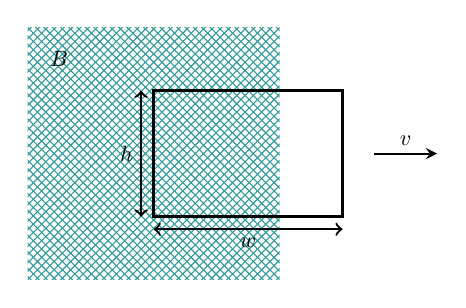
\begin{tikzpicture}[scale=0.8,every node/.style={scale=0.8}]
            \usetikzlibrary{patterns}
            \fill[pattern=crosshatch, pattern color=Teal!80] (0,0) rectangle (4,4);
            \node at (0.5,3.5) {\(\vetor{B}\)};
            \draw[very thick] (2,1) rectangle (5,3);
            \draw[thick, <->] (2,0.8) -- (5,0.8) node[midway,below] {\(w\)};
            \draw[thick, <->] (1.8,1) -- (1.8,3) node[midway,left] {\(h\)};
            \draw[-stealth, thick] (5.5,2) -- (6.5,2) node[midway,above] {\(\vetor{v}\)};
        \end{tikzpicture}
    \end{center}
    Suponha que a espira retangular, de lados \(h\) e \(w\), esteja se deslocando com uma velocidade constante \(\vetor{v}\), como indicado. Vimos em aula que a força eletromotriz total sobre o circuito da espira pode ser entendida como uma soma de dois termos,
    \begin{equation*}
        \varepsilon = \varepsilon_{\mathrm{fluxo}} + \varepsilon_{\mathrm{auto}} = - \diff{\Phi_{B}}{t} - L\diff{I}{t},
    \end{equation*}
    onde o primeiro termo diz respeito à variação do fluxo devido ao campo externo e o segundo à força eletromotriz induzida pela auto-indutância do próprio circuito, onde \(L\) é a auto-indutância da espira. Caso o fio tenha uma resistência interna \(R\), pode-se igualar \(\varepsilon = RI\) para obter uma equação diferencial para a função \(I(t)\). Contudo, caso possamos desprezar a resistência do fio, podemos igualar a força eletromotriz total a zero, significando que \(\varepsilon_{\mathrm{auto}} = -\varepsilon_{\mathrm{fluxo}}\). Nesse caso, calcule explicitamente \(\varepsilon_{\mathrm{fluxo}}\) em termos de \(\vetor{B}\), \(\vetor{v}\), \(h\), e do tempo \(t\), e encontre a corrente na espira \(I(t)\) para \(t > 0\). Considere que a espira começa a sair da região hachurada em \(t = 0\) e que \(I(0) = 0\). Faça um gráfico de \(I(t)\). Por fim, calcule a força magnética na espira devido ao campo externo em função do tempo.
\end{exercício}
\begin{proof}[Resolução]
    % Consideremos por ora uma corrente \(I'\) estacionária que percorre uma espira retangular de lados \(h\) e \(w\), então o campo magnético em um ponto \(\vetor{\x} = x\vetor{e}_x + y\vetor{e}_y\) contido na área delimitada pela espira é dado por
    % \begin{equation*}
    %     \begin{split}
    %         \vetor{B}(\vetor{\x}) &= \frac{\mu_0 I'}{4\pi} \left\{\int_0^w \dli{x'}\frac{\vetor{e}_x \times \left[(x - x')\vetor{e}_x + y\vetor{e}_y\right] }{\left[(x - x')^2 + y^2\right]^{\frac32}} + \int_0^h \dli{y'}\frac{\vetor{e}_y \times \left[(x - w)\vetor{e}_x + (y - y')\vetor{e}_y\right] }{\left[(x - w)^2 + (y - y')^2\right]^{\frac32}}\right.\\
    %                               &\hphantom{= \frac{\mu_0 I'}{4\pi}}\left. - \int_0^w \dli{x'} \frac{\vetor{e}_x\times\left[(x + x' - w)\vetor{e}_x + (y - h)\vetor{e}_y\right]}{\left[(x + x' -w)^2 + (y - h)^2\right]^{\frac32}} - \int_0^h \dli{y'}\frac{\vetor{e}_y\times\left[x\vetor{e}_x + (y + y' - h)\vetor{e}_y\right]}{\left[x^2 + (y + y' - h)^2\right]^{\frac32}}\right\}\\
    %                               &= \frac{\mu_0 I'}{4\pi} \vetor{e}_z\left\{\int_0^{w}\dli{x'}\frac{y}{\left[(x - x')^2 + y^2\right]^{\frac32}} - \int_0^h \dli{y'} \frac{x - w}{\left[(x - w)^2 + (y-y')^2\right]^{\frac32}}\right.\\
    %                               & \hphantom{= \frac{\mu_0 I'}{4\pi} \vetor{e}_z}\left. -\int_0^{w} \dli{x'}\frac{y - h}{\left[(x - x')^2 + (y - h)^2\right]^{\frac32}} + \int_0^h \dli{y'}\frac{x}{\left[x^2 + (y - y')^2\right]^{\frac32}}\right\}\\
    %                               &=\frac{\mu_0 I'}{4\pi}\vetor{e}_z \left\{ \int_0^\right\}
    %     \end{split}
    % \end{equation*}
    % A autoindutância da espira é dada por
    % \begin{equation*}
    %     L = \frac{\mu_0}{4\pi} \oint_{\Gamma} \dli{\vetor{\ell}}\cdot \oint_{\Gamma}\dli{\vetor{\ell'}} \frac{1}{\norm{\D}}
    % \end{equation*}

    Assumindo que a espira começa a sair da região com campo magnético no instante \(t = 0\), então o fluxo magnético pela espira é dado por
    \begin{equation*}
        \Phi_B(t) = \int_0^h \dli{y} \int_0^{w - v t} \dli{x} B = B h (w - v t)
    \end{equation*}
    sempre que \(t \in [0, \frac{w}{v}]\) e, portanto, a força eletromotriz induzida é
    \begin{equation*}
        \varepsilon_\mathrm{fluxo} = - \diff{\Phi_B}{t} = Bvh.
    \end{equation*}

    \begin{figure}[!ht]
        \centering
        \begin{tikzpicture}
            \def\B{1}
            \def\v{1}
            \def\h{1}
            \def\w{1}
            \def\L{1}
            \def\R{3}
            \begin{axis}[
                width=0.95\linewidth,
                height=0.2\textheight,
                xmin=0, xmax=1.15,
                ymin=0,ymax=1.2,
                domain=0:1,
                samples=1001,
                axis lines=middle,
                xlabel={\(t\)},
                xlabel style = {anchor=north east},
                % ylabel near ticks,
                ylabel={\(I(t)\)},
                legend pos=south east,
                ytick={0, \B*\v*\h/\R,(\B*\v*\v*\h)/\w},
                xtick={0,\w/\v},
                smooth,
                xticklabels={0, \(\frac{w}{v}\)},
                yticklabels={0,\(\frac{Bvh}{R}\),\(\frac{Bv^2h}{w}\)},
                ]
                \addplot[thick, Mauve] {\B*\v*\h*x/\L};
                \addlegendentry{\(R = 0\)};
                \addplot[thick, Pink, dashed] {(\B*\v*\h/\R)*(1 - exp(-(\R/\L)*x))};
                \addlegendentry{\(R \neq 0\)};
                \addplot[Pink!50,dotted] {\B*\v*\h/\R};
            \end{axis}
        \end{tikzpicture}
        \caption{Resposta indutiva perfeita e comparação com resposta indutiva com resistência não nula}
    \end{figure}

    Assim, a corrente induzida é dada por
    \begin{equation*}
        \diff{I}{t} = \frac{Bvh}{L} \implies I(t) = I(0) + \frac{Bvh}{L}t = \frac{Bvh}{L} t
    \end{equation*}
    onde \(L\) é a auto-indutância da espira.

    Com isso, a força magnética na espira devido ao campo é dada por
    \begin{equation*}
        \vetor{F} = \int_{w - vt}^{0} \dli{x} I(t) \vetor{e}_x \times \vetor{B} + \int_{h}^{0} \dli{y} I(t) \vetor{e}_y \times \vetor{B} + \int_{0}^{w - vt} \dli{x} I(t) \vetor{e}_x \times \vetor{B} = -B I(t) h \vetor{e}_x = -\frac{B^2 h^2 vt}{L}\vetor{e}_x,
    \end{equation*}
    desde que \(t \in [0, \frac{w}{v}]\).
\end{proof}
